\documentclass[11pt]{SANDreport}

%Local stuff
%\usepackage{latexsym}
%\usepackage[all]{draftcopy}

\usepackage{hyperref}
\usepackage{color}
\usepackage{graphicx}

\usepackage{listings}
\usepackage[compact]{titlesec}
\usepackage{mdwlist}

\usepackage{paralist}

%\usepackage{makeidx}
%\makeindex

%
% Command to print 1/2 in math mode real nice
%
\newcommand{\myonehalf}{{}^1 \!\!  /  \! {}_2}

%
% Command to print over/under left aligned in math mode
%
\newcommand{\myoverunderleft}[2]{ \begin{array}{l} #1 \\ \scriptstyle #2 \end{array} }

%
% Command to number equations 1.a, 1.b etc.
%
\newcounter{saveeqn}
\newcommand{\alpheqn}{\setcounter{saveeqn}{\value{equation}}
\stepcounter{saveeqn}\setcounter{equation}{0}
\renewcommand{\theequation}
	{\mbox{\arabic{saveeqn}.\alph{equation}}}}
\newcommand{\reseteqn}{\setcounter{equation}{\value{saveeqn}}
\renewcommand{\theequation}{\arabic{equation}}}

%
% Shorthand macros for setting up a matrix or vector
%
\newcommand{\bmat}[1]{\left[ \begin{array}{#1}}
\newcommand{\emat}{\end{array} \right]}

%
% Command for a good looking \Re in math enviornment
%
\newcommand{\RE}{\mbox{\textbf{I}}\hspace{-0.6ex}\mbox{\textbf{R}}}

%
% Commands for Jacobians
%
\newcommand{\Jac}[2]{\displaystyle{\frac{\partial #1}{\partial #2}}}
\newcommand{\jac}[2]{\partial #1 / \partial #2}

%
% Commands for Hessians
%
\newcommand{\Hess}[2]{\displaystyle{\frac{\partial^2 #1}{\partial #2^2}}}
\newcommand{\hess}[2]{\partial^2 #1 / \partial #2^2}
\newcommand{\HessTwo}[3]{\displaystyle{\frac{\partial^2 #1}{\partial #2 \partial #3}}}
\newcommand{\hessTwo}[3]{\partial^2 #1 / (\partial #2 \partial #3)}



%\newcommand{\Hess2}[3]{\displaystyle{\frac{\partial^2 #1}{\partial #2 \partial #3}}}
%\newcommand{\myHess2}{\frac{a}{b}}
%\newcommand{\hess2}[3]{\partial^2 #1 / (\partial #2 \partial #3)}

%
% Shorthand macros for setting up a single tab indent
%
\newcommand{\bifthen}{\begin{tabbing} xxxx\=xxxx\=xxxx\=xxxx\=xxxx\=xxxx\= \kill}
\newcommand{\eifthen}{\end{tabbing}}

%
% Shorthand for inserting four spaces
%
\newcommand{\tb}{\hspace{4ex}}

%
% Commands for beginning and ending single spacing
%
\newcommand{\bsinglespace}{\renewcommand{\baselinestretch}{1.2}\small\normalsize}
\newcommand{\esinglespace}{}


\setcounter{tocdepth}{3}

\raggedright

% If you want to relax some of the SAND98-0730 requirements, use the "relax"
% option. It adds spaces and boldface in the table of contents, and does not
% force the page layout sizes.
% e.g. \documentclass[relax,12pt]{SANDreport}
%
% You can also use the "strict" option, which applies even more of the
% SAND98-0730 guidelines. It gets rid of section numbers which are often
% useful; e.g. \documentclass[strict]{SANDreport}

% ---------------------------------------------------------------------------- %
%
% Set the title, author, and date
%

\title{\center
Trilinos Lifecycle Model \\[2ex] Version 2.0 \\[2ex] \large A
Lean/Agile Software Lifecycle Model for Research-based Computational
Science and Engineering and Applied Mathematical Software }
\author{
Roscoe A. Bartlett \\ Oak Ridge National Laboratories\footnote{Oak
Ridge National Laboratories is Managed by UT-Battelle, a partnership
of the University of Tennessee and Battelle Memorial Institute, for
United States Department of Energy under Contract DE-AC05-00OR22725.} 
\\[2ex] Mike Heroux \\ Roger Pawlowski \\ Jim Willenbring \\ Sandia
National Laboratories\footnote{Sandia is a multiprogram laboratory
operated by Sandia Corporation, a Lockheed-Martin Company, for the
United States Department of Energy under Contract DE-AC04-94AL85000.},
Albuquerque NM 87185 USA, \\ }
\date{}

% ---------------------------------------------------------------------------- %
% Set some things we need for SAND reports. These are mandatory
%
\SANDnum{SAND2011-XXXX}
\SANDprintDate{November ???}
\SANDauthor{
Roscoe A. Bartlett \\ Mike Heroux \\ Roger Pawlowski \\ Jim
Willenbring }

% ---------------------------------------------------------------------------- %
% The following definitions are optional. The values shown are the default
% ones provided by SANDreport.cls
%
\SANDreleaseType{Unlimited Release}
%\SANDreleaseType{Not approved for general release}

% ---------------------------------------------------------------------------- %
% The following definition does not have a default value and will not
% print anything, if not defined
%
%\SANDsupersed{SAND1901-0001}{January 1901}

%
% Glossary
%

%\makeglossaries
%\newglossaryentry{value_type}{name={Value Type},
%description={A concrete built-in or user-defined (class) type that has a
%public default constructor, copy constructor, and assignment operator.  Value
%type objects typically have a small memory footprint which allows them to be
%copied without excessive overhead.}


% ------------------------------------------------------------------------- %
%
% Start the document
%
\begin{document}

\pagenumbering{roman}

\maketitle

% ------------------------------------------------------------------------ %
% An Abstract is required for SAND reports
%

%
\begin{abstract}
%

Software lifecycle is becomming an increasing important issue for
computational science \& engineering (CSE) and applied mathematical
software.  The process by which a piece of CSE software begins life as
a product of a research effort and then matures into a trusted
high-quality capbility is a vexing problem for the CSE community.
Here we describe a proposal for a well-defined software lifeycle
processs based on modern Lean/Agile software engineering priciples
that is appropriate for many CSE software projects that are initally
heavily focused on research but also are expected to be eventually
produce usable high-quality capabilities.  Here, four different phases
are suggested for the transition from research to production software
that consider the appropriate handling of many issues such as level of
clarity of the code base, testing, user documentation, user error
handling and feedback, and backward compatibility.  In particular, a
specific regulated backward compatibiliy process is described as well
as the notion of ``self-sustaining software''.  An important
collection of software in this domain is Trilinos which is used as the
motivation and the initial target for this lifecycle model.  However,
many other related and similar CSE (and non-CSE) software projects
might also make good use of this model.  Indeed this lifecycle
process, if followed, would allow for very large-scale sustainable
integration of large amounts of complex CSE software efforts across
many different institutions.

%
\end{abstract}
%

% ------------------------------------------------------------------------ %
% An Acknowledgement section is optional but important, if someone made
% contributions or helped beyond the normal part of a work assignment.
% Use \section* since we don't want it in the table of context
%
%\clearpage
%\section*{Acknowledgment}
%
%
%The format of this report is based on information found
%in~\cite{Sand98-0730}.

% ------------------------------------------------------------------------ %
% The table of contents and list of figures and tables
% Comment out \listoffigures and \listoftables if there are no
% figures or tables. Make sure this starts on an odd numbered page
%
\clearpage
\tableofcontents
%\nopagebreak\listoffigures
%\nopagebreak\listoftables

% ---------------------------------------------------------------------- %
% An optional preface or Foreword
%\clearpage
%\section{Preface}
%Although muggles usually have only limited experience with
%magic, and many even dispute its existence, it is worthwhile
%to be open minded and explore the possibilities.

% ---------------------------------------------------------------------- %
% An optional executive summary
%\clearpage
%\section{Summary}
%Once a certain level of mistrust and scepticism has
%been overcome, magic finds many uses in todays science
%and engineering. In this report we explain some of the
%fundamental spells and instruments of magic and wizardry. We
%then conclude with a few examples on how they can be used
%in daily activities at national Laboratories.

% ---------------------------------------------------------------------- %
% An optional glossary. We don't want it to be numbered
%\clearpage
%\section*{Nomenclature}
%\addcontentsline{toc}{section}{Nomenclature}
%\begin{itemize}
%\item[alohomora]
%spell to open locked doors and containers
%\end{itemize}

% ---------------------------------------------------------------------- %
% This is where the body of the report begins; usually with an Introduction
%
\SANDmain % Start the main part of the report

\pagenumbering{arabic}

%
\section{Introduction and Background}
%

Computational Science and Engineering (CSE) is experiencing a
challenge in software lifecycle issues.  Much software in CSE begins
development as research software but at some point begins to be used
in other software and is desired (or is expected) to eventually
achieve production-quality.  There is currently no sufficient software
engineering lifecycle model defined for these types of CSE software
that has been shown to be effective and/or to actually be followed.  A
previous attempt to create a viable lifecycle model for Trilinos to
provide for transitions of CSE software from research, to production,
to maintenance (and later death) was defined in
{}\cite{TrilinosLifecycleModel2007}.  However, as of 2011, there have
been no examples of the successful full execution of this lifecycle
model on any Trilinos package and no signs that it will be followed by
any of the Trilinos package teams to produce production-quality CSE
software (i.e. the ``Production Maintenance'' phase) using that
lifecycle model.

What is needed is a new Lean/Agile-consistent lifecycle model for
research-driven CSE software that can provide a smooth transition from
research to production and provide the needed level of quality for
every lifecycle phase along the way.  In order to define such a
lifecycle model it is likely that research software will need to be
developed right from the beginning at a higher than average level of
quality in a Lean/Agile consistent way with better unit and
verification tests.  These tests will need to be developed right from
the beginning and the internal structure of the software will need to
be maintained at higher quality using Agile/Emergent design and
Continuous Refactoring.  Such lifting of the quality of basic research
software is needed just from the standpoint of creating credible
research results that are suitable for publication in peer-reviewed
journals {}\cite{CompSciDemandsNewParadigm05,
ScientistsNightmareFiveRetractions2006}.

ToDo: Give some type of overview of Lean and Agile and why they are
important.

In this current document, we try to define a new lifecycle model for
Trilinos and related CSE software that will become the standard across
the Trilinos effort and related projects.

ToDo: Give an outline for the rest of the document.


%
{}\section{Current State of Trilinos Software Engineering}
\label{sec:trilinos_current_state}
%

Before describing the new Trilinos lifecycle model it is worthwile to
set the context of the current state of Trilinos software engineering
and development practices.  These pracitices and policies are
ingrained into the Trilinos development environment and are taken for
granted in this disucssion for a new Trilinos lifecycle process.

The short list of Trilinos software engineering processes and
practices include:
%
\begin{compactitem}
%
{}\item official separation of Trilinos code into Primary
Stable (PS), Secondary Stable (SS), and Experimental (EX) for testing
purposes
%
{}\item increasingly more extensive automated nightly regression and
portability testing of PS and SS Code
%
{}\item synchronous CI (pre-push) testing of PS code using the Python
tool checkin-test.py
%
{}\item asynchronous CI (post-push) testing of SS code using
package-based CTest driver posting to CDash
%
{}\item strong policies on the maintenace of 100\% clean PS and SS
builds and tests
%
{}\item Regular quarterly releases of Trilinos.
%
\end{compactitem}

The official segregation of (Primary and Secondary) Stable Code from
Experimental code in Trilinos has allowed the Trilinos development
team to define and enforce fairly rigorous policies on keeping Stable
code building and having all the tests of Stable features run
successfully.  This is maintained through the synchrounous CI
(pre-push) and asynchronous CI (post-poss) testing tools and processes
and strong peer pressure to keep PS and SS code build and tests 100\%
clean.  However, with respect to lifecycle, having 100\% clean tests
means very little if your test coverage is low (which is the case in
many existing Trilinos packages).  Technically speaking, Stable Code
with test coverage not near 100\% at all times means the code is not
meeting basic Agile development standards (see {}\cite{XP2} and
{}\cite{CodeComplete2nd04}).  Note, however, that the distiction
between PS, SS, and EX code in Trilinos has to do with the commitment
of the development team to maintain (or not in the EX case) the status
of builds and passing tests on various platforms and has nothing to do
with the assumed quality of the software.  Official assignments and
metrics of software quality in Trilinos are currently non-existent.


%
{}\section{Overview of a New Trilinos Software Lifecycle Model}
\label{sec:life_cycle_overview}
%

Here, we propose a lifecycle model with four possible phases.  The
concepts of ``self-sustaining software'' and ``regulated backward
compatibility'', which are critical in the defintion and goals of
these phases, are described in
Section~\ref{sec:regulated_backard_compatibility} and
Section~\ref{sec:self_sustaining_open_source_software}, respectively.

The four proposed lifecycle phases are:

\begin{compactenum}

{}\item Purely Experimental Code:

\begin{compactitem}

{}\item generally {}\underline{not} developed in a Lean/Agile
consistent way,

{}\item does not provide sufficient unit (or otherwise) testing to
prove correctness,

{}\item could actually be declared to be Secondary Stable code with
respect to CI and nightly Trilinos testing but in general would be
considered to be untested Experimental code in Trilinos,

{}\item no one should use such code for anything important (not even
for research results but in the current CSE environment publication
using such software would likely still be allowed),

{}\item generally should {}\underline{not} go out in general releases
of Trilinos, and

{}\item does {}\underline{not} provide a direct foundation for
creating production-quality code.

\end{compactitem}

{}\item Research Stable Code:

\begin{compactitem}

{}\item developed in a Lean/Agile consistent way,

{}\item strong unit and verification tests (i.e.\ proof of
correctness) written as the code/algorithms are being developed
(should have almost 100\% line coverage at the very least),

{}\item could be Primary Stable or Secondary Stable code in Trilinos,

{}\item generally does {}\underline{not} have good examples,
documentation, etc.,

{}\item appropriate to be used only by ``expert'' users,

{}\item appropriate to be part of a general release,

{}\item appropriate to be used only in ``friendly'' customer codes,

{}\item would tend to provide for some regulated backward
compatibility but may not, and

{}\item provides a strong foundation for creating production-quality
software.

\end{compactitem}

{}\item Production Growth Stable Code:

\begin{compactitem}

{}\item includes all the good qualities of ``Research Stable Code'',

{}\item provides increasingly improved validation of user input errors
and better error reporting,

{}\item has increasingly better formal documentation (Doxygen,
technical reports, etc.),

{}\item has increasingly better examples, tutorial material, etc.,

{}\item maintains clean structure through refactoring of the code and
user interfaces to make more consistent, easier to maintain etc.,

{}\item maintains increasingly better regulated backward compatibility
with few (if any) truly incompatible changes with new releases,

{}\item expands in usage in more customer codes, and

{}\item is appropriate to turn over to a maintenance support team near
the end of the stage.

\end{compactitem}

{}\item Production Maintenance Stable Code:

\begin{compactitem}

{}\item includes all the good qualities of ``Production Growth Stable
Code'',

{}\item primary development includes mostly just bug fixes and
performance tweaks,

{}\item maintains rigorous backward compatibility with typically no
deprecated features or any breaks in backward compatibility, and

{}\item could be maintained by parts of the user community if
necessary (i.e.\ as ``self-sustaining software'').

\end{compactitem}

\end{compactenum}

{}\textbf{ToDo:} Create a chart showing the how testing, documentation
and tutorials, design and code clarity, defects, quality of user error
feedback, backward compatibility, usage in customer code

One should start developing software right from the beginning as
``Research Stable Code''.  The ``Purely Experiment Code'' category
really should not exist in a Lean/Agile consistent lifecycle model but
is needed as a catch-all for code that lacks the level of unit and
verification testing or level of clarity and simplicity needed to be
considered consistent with Lean/Agile software.  The level of examples
or other documentation can be in very different stages of maturity yet
the software can still be considered very good Lean/Agile software.
What differentiates Lean/Agile ``Research'' software from Lean/Agile
``Production-quality'' software is not the amount of testing and proof
of correctness but instead is the level of user (and developer)
documentation, input validation and error reporting, and perhaps the
polish of the interfaces.  However, even ``research'' software will
tend to have a clean internal structure and have reasonably consistent
user interfaces if it is developed using good Lean/Agile practices
(including Emergent Design and Continuous Refactoring).

Related to the issue of the Trilinos lifecycle process is whether or
not the Trilinos project will take an official position on trying to
provide a minimum level of quality for packages provided in a general
release.  On one extreme, the Trilinos project may provide no
guarantees at all and it is up to the users of Trilinos to determine
the level of quality with respect to each and every Trilinos package
on their own and decide which packages to use and which packages to
shy away from.  On the other extreme, the Trilinos project could
demand a minimum level of quality in order for a package to be part of
an official Trilinos release.  Other packages could provide
``unofficial'' releases if they would like on their own terms.  This
is an important issue to address to define what Trilinos really is.
Is Trilinos just a container for a lot of independently developed
software that can be used together in some cases (the former view) or
is Trilinos a coordinated effort to create high-quality CSE software
(the latter view).

Note that issues like version-control, automated testing, nightly and
continuous integration testing, and other basic extremely well
aceepted software technical practicies are already intimately woven
into the Trilinos devleopment community (see
Section~\ref{sec:trilinos_current_state}).  These policies and
practicies, while very important, do not directly impact a lifecycle
mode except to make it easier and safer to implement.  Therefore, we
will not discuss such basic software practices and policies in this
document except where needed and instead refer the reader to the
Trilinos Developers Website and the references for details.

Before describing the four different phases of this new Trilinos
lifecycle model in more detail, the important concepts of
``self-sustaining software'' and ``regulated backward compatibility''
are defined in the next two sections.


%
{}\section{Self-Sustaining Open-Source Software: Defined}
\label{sec:self_sustaining_open_source_software}
%

The CSE domain is a complex and challenging domain for the development
and sustainability of high-quality software.  Many CSE projects have
development and usage lifetimes that span 10 to 30 years or more.
These projects have to port to many different platforms over their
lifetime as computing technology shifts and the software must be
augmented and changed as new and better algorithms are developed
{}\cite{HPCNeedsAToolsStrategy05}.  In such an environment, creating a
strong dependence on commersial tools and libraries can be a large
risk.  Companines are purchased and product lines go away (e.g. Intel
purchased the KAI C++ compiler and killed it and it took years before
the Intel compilers reached the same level of quality as the KAI C++
compiler in compiling deeply templated C++ code).  In addition,
complex non-commersial software produced in the U.S. national
laboratories and universities which require continuing development,
maintenance and support teams also represent a risk to long-lived CSE
projects.  For example, what happens to customer projects that adopt a
complex SciDAC software library when the funding goes away which
removes the associated supporting SciDAC-funded development and
support team?

What we advocate here is that CSE software like Trilinos packages that
will be used by other CSE projects needs to be developed in such a way
as to be ``self-sustaining'' such that customer project teams could
take over the basic maintance and support of the software for their
own use if needed.

We hereby define Self-Sustaining Software as software with the
following properties:
%
\begin{compactitem}

{}\item\textit{Open-source}: The software has a sufficiently loose
open-source license allowing the source code to be arbitraily modified
and used and reused in a variety of contexts (including unrestricted
usage in comersial codes).

{}\item\textit{Core domain distillation document}: The software is
accompanied with a short focused high-level document describing the
purpose of the software and its core domain model
{}\cite{DomainDrivenDesign}.

{}\item\textit{Exceptionally well testing}: The current functionality
of the software and its behavior is rigorously defined and protected
with strong automated unit and verification tests.

{}\item\textit{Clean structure and code}: The internal code structure
and interfaces are clean and consistent.

{}\item\textit{Properties apply recursively to upstream software}: All
of the external upstream software that are depended on are also
themselves self-sustaining software as so on.

{}\item\textit{All changes done in a way to maintain these
properties}: All maintenance of the software maintains all of these
properties of self-sustainingsoftwarwe (by applying Agile/Emergent
Design and Continuous Refactoring and other good Lean/Agile software
development practicies).

\end{compactitem}

The software must be open source so that customer projects can make
needed changes to the software to suite needs and do critical porting
work.  Non-open-source commercial software relies on the supplying
vender to make needed modifications and porting which they might not
be able to do for various reasons.  Also, the open-source license must
be open enough to allow broad reuse.  For example, LGPL is okay for
many organizations but some organziations (such a commersial and even
some private for-profit companies) cannot use LGPL software.  GPL
software is also inappropriate for self-sustaining CSE software by any
reasonble measure.  However, the BSD license seems to be open enough
to allow no restructions on use and reuse and should therefore be
preferred as the default open-source license for self-sustaining
software.

A high-level document is needed to define the scope and the high-level
goals and core domin of the software needed to maintain the
``conceptual integrety'' of the software~\cite{MythicalManMonth95}.
This document will be short and focused and will define the high-level
``Core Domain Model'' for the particular piece of CSE
software~\cite{DomainDrivenDesign}.  An example of a domain model for
a multi-physics coupling package is given in {}\cite{LIMEtheory}.

As or more important than a high-level domain-model document is a
strong set of unit and verification tests.  Such tests are critical in
order to allow the software to be safely and efficiently changed to
add new features, port to new platforms, and generally refactor the
code as needed without breaking behavior or destroying backward
compatibility (see {}\cite{WorkingEffectivelyWithLegacyCode05}).  Of
course, code with strong unit and verification tests will have very
few defects (i.e.\ in Agile, there are no defects, only missing
tests).  Such a testing foundation needs to be put in place from day
one as the first lines of code are written (preferabily using
Test-Drive Development (TDD) {}\cite{TDD}).  Any software lifecycle
model and process that does not include strong unit and verification
testing from the very beginning of the project is not Lean/Agile
consistent and cannot be used as the foundation for eventually
producing trusted production-quality software.

Maintaining a clean and simple internal structure of the code is
crtial for achieving self-sustaining software.  No matter how good the
unit and verification tests are, if the code is too convoluted and/or
has too many entangling dependencies and tricky behaviors, the
software will not be able to be affordably maintained to port to new
platforms or changed for other purposes.  Developing software which
keeps a clean internal structure can only be done using continuous
refactoring and redesign {}\cite{XP2}.  Without applying such a
skilled and rigorous process for maintaining the software, under
maintenance and futher development it will eventually die the slow
death of ``software entropy'' and become unsustinable
{}\cite{MythicalManMonth95}.

Developing software of this type requires a high degree of skill and
knowledge and places a very high standard on CSE development teams
which first create and later maintain the software.

Also, it is not enough for a given piece of software to satisfy the
basic properties of self-sustaining software, but it is also critcial
that the dependencies of self-sustaining software also themselves be
self-sustaining software. Therefore, the defintion of self-sustaining
software is recursive in nature.  For example, suppose a piece of
software is clear and well tested but has a critcial dependency on a
comersial numerical library that is unique and not easy to replace.
If the vender removes support for this critical comersial numerical
library, the downstream open-source software may become unusable and
non-portable to future platforms.

Any software that does not maintain these properties as it is ported
and maintained will slowly (or rapidly) become unsustainable which
then becomes a liabiliy to the various customer CSE software projects.
Again, this is a high bar to define for CSE software developers but it
critical if one is serious about sustainable large-scale CSE software
integration.

Note that self-sustaining software does not necessarily have good user
documenation, really any user-oriented examples, nor necessarily
produce good error messages for invalid user input.  While these
properties of any piece of software are important for the adoption and
usage of software they do not affect the sustainabiliy of the software
by an existing set of client projects.  The tests define the expected
behavior of the software that must be maintained (or purpusfully
changed by changing the tests).


%
{}\section{Regulated Backward Compatibility}
\label{sec:regulated_backard_compatibility}
%

Backward compatibility is a central issue in Agile software
development.  The issue of regulated backward compatbility was
mentioned in Section ??? and is a critical aspect of CSE software used
by other projects.  First, the paradox of backward compatbility in
Agile software devlopment is discussed and then the official Trilinos
strategy for regulated backward compatibility is described.


%
{}\subsection{The Paradox of Backward Compatibility and Constantly
Changing Agile Software}
\label{sec:paradox_of_back_compat_agile}
%

Agile software is iteratively developed and released to cutomers with
very early releases preferably contining very little initial
functionality followed my many frequent releases with more and more
functionality {}\cite{AgileSoftwareDevelopment}.  All the while, the
software is constantly being refactored and refined with each new
release.  Software developed in an Agile way needs early and frequent
feedback from real customers.  Without that early and frequent
feedback from real customer usage, Agile methods fundamentally fall
apart and cannot operate.

However, most perspective customers are usually not very interested in
starting to adopt and use a piece of software that is constantly
changing with every new iterative release.  Interface changes in
aggressively developed software break customer code and require the
customer developers to constantly be chasing changes, dealing with
broken builds and changing behavior.  Most customers would rather wait
until the perspective software ``stablizes'' before deciding to start
using the software (and therefore start giving feedback).  But here in
lies the paradox; Agily developed software cannot stabilize its
interfaces and behavior unless customers use the software and give
feedback after many iterations of releases but customers do not want
to adopt software that is constantly changing.

So if customers do not want to use software that is constantly
changing and Agily devleoped software cannot stabilize unless its gets
feedback from customer usage, how can we actually develop Agile
software without placing an unreasonble burden on customers?  The
answer is to carefully manage changes in Agily devloped software
interfaces and behavior and smooth the transition for customers to
make upgrades of iterative (or continuous) releases as easy, safe, and
painless as possible.  The way we do that is to adopt a riggorous set
of policies and practicies for {}\textit{regulated backward
compatibility}.


%
{}\subsection{The Need for Backward Compatibility}
\label{sec:need_for_back_compat}
%

Backward compatibility is critical for safe upgrades of new releases
of software and for the composability and compatibility of different
software collections.  If every new release of a piece of software
breaks backware compatibility, it discurages users from depending on
the software or discourages doing upgrades.  In the case of CI, if a
package constantly is breaking backward compatibiliy, downstream
packages must constantly be updated to keep up, making for a difficult
and inefficient development process.  In the case of composability of
software through releases, some backward compatibility is critical to
allow for different collections of software to be integrated.

\begin{figure}
\begin{center}
%\fbox{
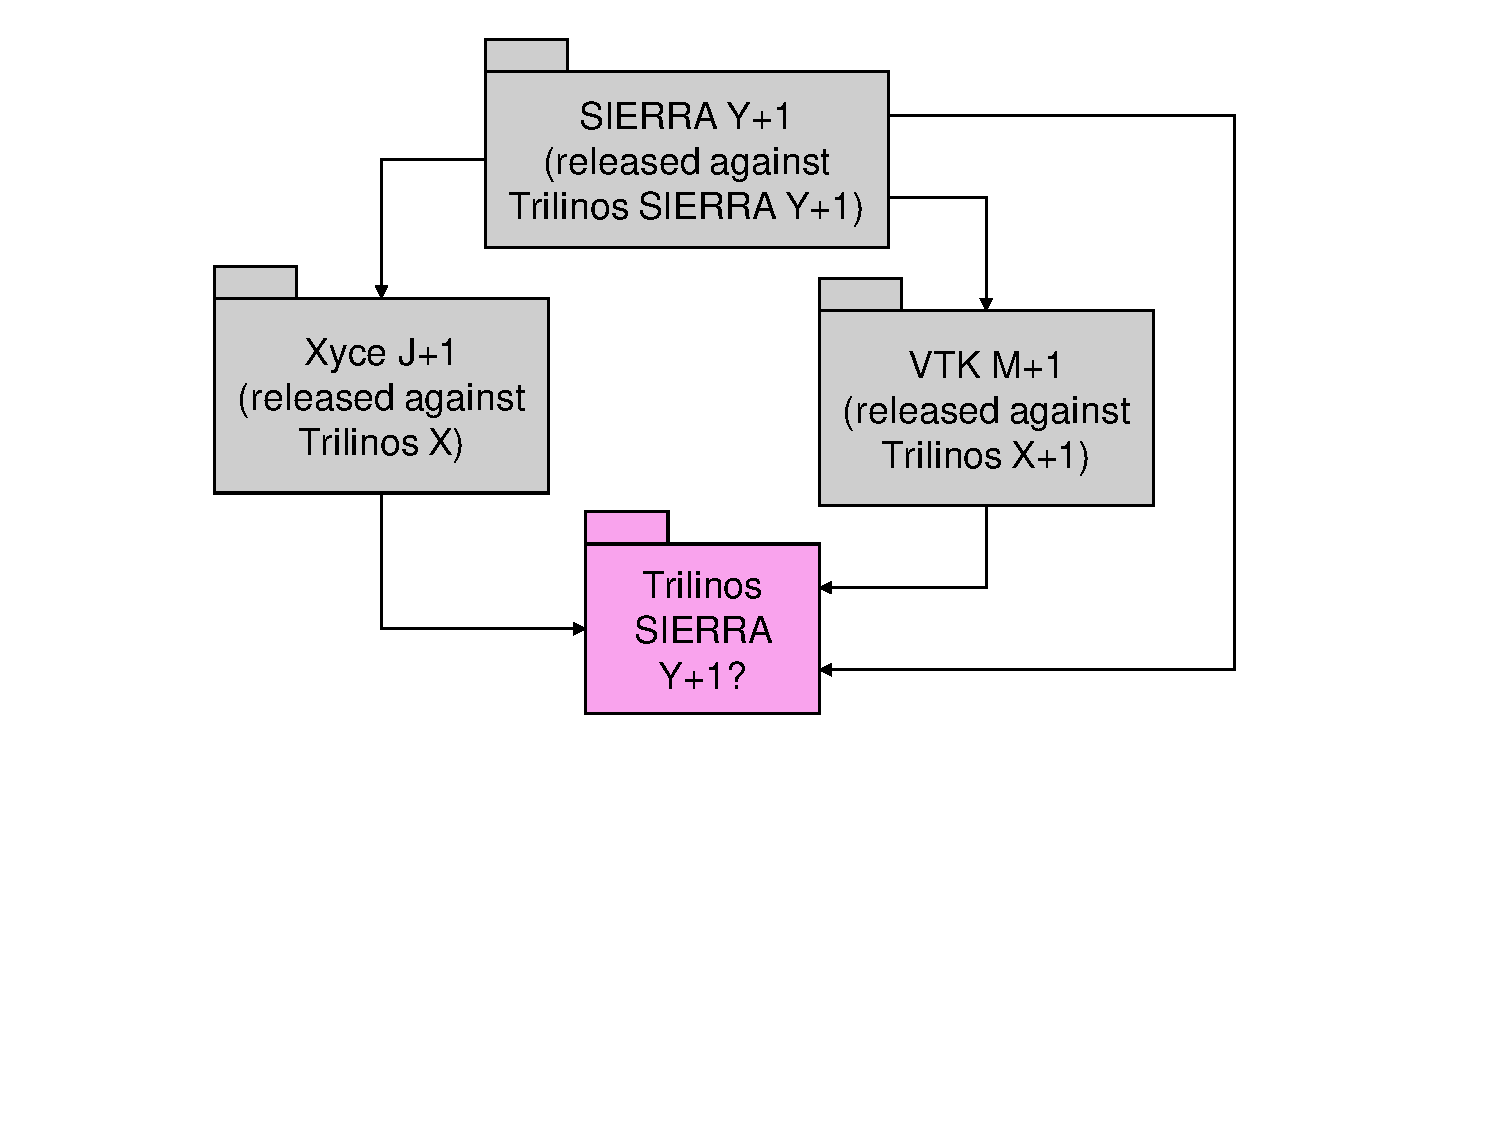
\includegraphics[trim = 1.0in 2.7in 1.0in 0.2in, scale=0.55]
{XyceSierraVtkTrilinosCompatibility}
%}
\caption{
Demonstration of the need for backward compatiblity for multiple
releases.}
\label{fig:XyceSierraVtkTrilinosCompatibility}
\end{center}
\end{figure}

ToDo: Describe the Xyce, SIERRA, VTK, Trilinos example for why we need
some backward compatibility.  Show the diagram and describe it.


%
{}\subsection{The Cost of Maintaining Backward Compatibility}
\label{sec:costs_of_back_compat}
%

While maintaining some backward compatibility is a critical
requirement for large scale development and software integration (in
CI or through relases) as described above, maintaining backward
compatibility also comes with potentially high costs over a long lived
project.  The main costs are the extra testing needed to prove
backward compatibility and the cost of the accumulation of technical
dept that occurs because of the inability or extra cost to refactor
software.

As new features are developed and new interfaces are created,
maintaining backward compatibility requires keeping older versions of
classes and functions around with the old behavor.  Keeping around the
old interfaces and functionality bloats the code base and requires
more code to build and more tests to run an maintain.  This overhead
of the extra code to maintain, build, and test taxes the entire
development effort.  Dropping backward compatibility, however, allows
for deleting old obsolete software and tests and makes the entire
development effort run faster.

Also, the extra cost in maintaining old interfaces and behavior as new
behavior is created discurages the creation of new interfaces and
classes.  Instead of changing existing interfaces (which would break
backward compatibility), developers are draw to keep the same
interfaces in place and then put in work-arounds to add new behavior.
Often these tweeks are not done in a clean way and the resulting
software becomes messier and more and more lacks consistent structure.
This tendency of software under subsequent releases and modifications
to loose its internal structure was refereed to as ``software
entropy'' in {}\cite{MythicalManMonth95}.  Without constant
refactoring to clean up the interfaces and design of the software
(which often breaks backward compatibility), such software dies a slow
death of rising ``technical debt''
{}\cite{ImplementingLeanSoftwareDevelopment}.  When backward
compatibility is not maintained, then the software can be freely
refactored to maintain ``conceptual integrity''
{}\cite{MythicalManMonth95}.

Therefore, while it is easy to see the critical need for maintaining
some backward compatibility as desctibed in
Section~\ref{sec:need_for_back_compat}, we have also acknowledged that
maintaining backward compatibility over a long lived piece of software
can impart significant extra cost and/or signficantly increse the
``software entroy'' and ``technical debt'' of the software that will
eventually make the software unable to continue to be changed from a
cost/benefit point of view.

%
{}\subsection{Regulated Backward Compatibility: Defined}
\label{sec:defined_reg_back_compat}
%

ToDo: Describe X.Y.X numbering

\begin{verbatim}
Trilinos Version Numbering X.Y.Z:
X: Defines backward compatibility set of releases
Y: Major release (off the master branch) number in backward compatible set
Z: Minor releases off the release branch X.Y
Y and Z: Even numbers = release, odd numbers = dev
Makes logic with Trilinos_version.h easier
Backward comparability between releases:
Example: Trilinos 11.6 is backward compatible with 11.0 through 11.4
Example: Trilinos 12.I is not compatible with Trilinos 11.J
\end{verbatim}

\begin{figure}
\begin{center}
%\fbox{
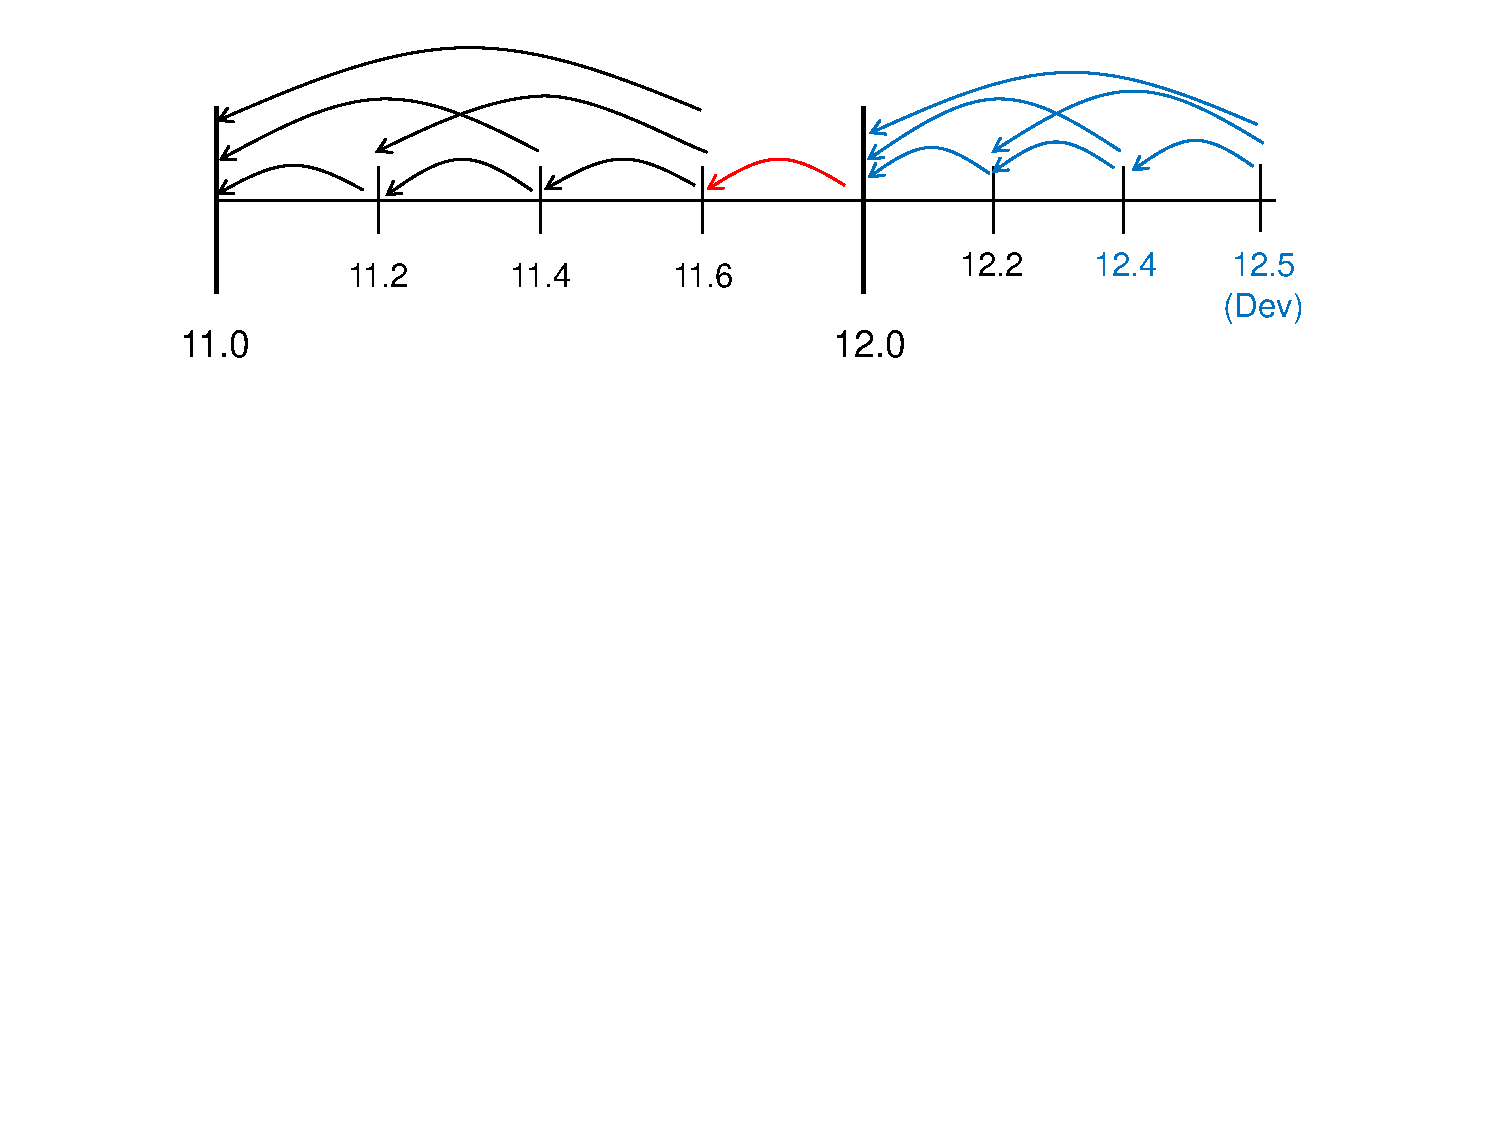
\includegraphics[trim = 1.0in 5.0in 1.0in 0.2in, scale=0.55]
{BackwardCompatibilityTimeline}
%}
\caption{
Release backward compatibiliy timeline.}
\label{fig:BackwardCompatibilityTimeline}
\end{center}
\end{figure}

ToDo: Describe backward compatibility timeline figure.

ToDo: Fill in!


%
{}\subsection{Regulated Backward Compatibility: Details}
\label{sec:details_reg_back_compat}
%

\begin{verbatim}
A compromise: Regulated backward compatibility (Trilinos approach)
Maintain a window of ``sufficient'' backward compatibility over major version numbers (e.g. 1-2 years)
Provide �Deprecated'' compiler warnings
Example: GCC's __deprecated__ attribute enabled with
-DTrilinos_SHOW_DEPRCATED_WARNINGS:BOOL=ON
Drop backward compatibility between major version numbers
[Future] Provide strong automated testing of Trilinos backward compatibility
\end{verbatim}

Guidelines for breaking backward compatibility:

\begin{itemize}

{}\item\textit{Prepair users for the break in backward compatibility}:
Try to to provide some preparation for breaking backward compatibility
in previous releases.  The best way to do this is to mark code as
``deprecated''.  The GCC and Intel C++ compilers support a
{}\ttt{\_\_deprecated\_\_} propertly that can provide compile-time
deprecated warnings.  There are many strategies for approprtiately
deprecating code to allow users a means to perfom smooth transitions
to new functionality even before

{}\item\textit{Fail big and hard when backward compatibility is
dropped}: When breaking backward compatiblity, client code should
break in an obvious way.  Ideally, non-upgraded client code should not
even compile and the compile errors should be as obvious as possible.
If compile errors are not possible, link-time errors would be the next
best alterative.  If build errors are not possible, then runtime
errors should be generated with good error messages helping the user
to know what needs to be changed.

{}\item\textit{Provide for safe straightforward upgrades}: When
breaking backward compatibility, try to provide the user an easy and
error-proof approach to upgrade their code.  For example, if changing
the name of a set of classes and functions, provide a sed-like script
that the user can run on their code to preform the name changes.  This
can be difficult for raw class and function names.  However, for
globally unique identifiers (like macro names)

\end{itemize}

Guidelines for deprecating functionality:

\begin{itemize}

{}\item Deprecate classes and functions using the standard
{}\ttt{<UCPACAKGENAME>\_DEPRECATED} macro.

{}\item Deprecate macros by by calling dummy deprecated functions
using the standard {}\ttt{<UCPACAKGENAME>\_DEPRECATED} macro.

\end{itemize}


%
{}\section{Detailed Discussion of the Proposed Lifecycle Stages}
%

Now that that four different lifecycle phases have been introduced and
the concepts of self-sufficient software and regulated backward
compatibility have been descripted, here the four different lifecycle
phases are discussed in more detail.


%
{}\subsection{Purely Experimental Code}
%

As mentioned in Section~\ref{sec:life_cycle_overview}, the Purely
Experimental Code stage is a place-holder for any research software
that has not been developed in a Lean/Agile consistent way and is not
an approriate direct foundation for later development of
production-quality software.  For example, software with very low
coverage of testing can likely not be considered to be Stable
software.

This stage could also be used for other non-research software that
might otherwise be considered production-quality software by some yet
lacks many key attributes of self-sustaining software.  Such
non-Lean/Agile consistent software will not be discussed further here
except to acklowlege that such software exists in abundance in the CSE
community (and yes also in many current Trilinos packages).

However, all hope is not lost when dealing with Purely Experimental
software.  Nearly any piece of software can have unit tests developed
and can be refactored into a quality piece of software given enough
time and effort.  For example, the appraoches described in
{}\cite{WorkingEffectivelyWithLegacyCode05} can be used to methodically
and safely alter such software into what might be considered Stable
Code, as defined in the following lifecycle stages.


%
{}\subsection{Research Stable Code}
%




ToDo: Fill in!


%
{}\subsection{Production Growth Stable Code}
%

ToDo: Fill in!


%
{}\subsection{Production Maintenance Stable Code}
%

ToDo: Fill in!


%
{}\section{Risk Analysis and Acceptance Testing}
\label{sec:risk_analysis}
%

ToDo: Fill in ...


%
\section{Grandfathering of Existing Trilinos Packages}
%

At the time of this writing, many of the established long-released
Trilinos packages don't even meet the criteria for ``Research Stable
Code''.  However, some of these established Trilinos packages are
hardened through extensive use by customers and bug fixes and they are
not as actively developed and therefore certain common use-cases are
well verified.  This is a typical way in which verification testing is
performed in CSE and other domains but is not Lean/Agile consistent
and does not lead to self-sustaining software.  We will have to
``forgive'' this current generation of Trilinos packages and
grandfather them into a new lifecycle model.  However, we will need to
work hard to make sure the next generation of Trilinos packages do
better (and fix some of the existing packages that will be part of the
next-generation of Trilinos and will be continued to be developed at
some level).

ToDo: Finish this!


%
\section{Comparison to the Previously Defined Trilinos Lifecyle Model}
%

ToDo: Outline the old Trilinos lifecycle mode here.

One key difference between the new lifecycle phases and the Trilinos
lifecycle phases given in {}\cite{TrilinosLifecycleModel2007} is that
the transition from ``research'' to ``production'' does not involve
the ``hardening'' of the functioning of the software or a complete
rewrite of the software (which is never going to happen, see below)
which is required in the promitional event for going from ``Production
Growth'' to the ``Production Maintenance'' phases in the original
Trilinos lifecycle model.  There are no modern SE lifecycle processes
that advocate this type of approach to developing software.  There is
likely not even a single Trilinos package that meets the criteria for
the ``Phase 2: Production Growth'' phase in
{}\cite{TrilinosLifecycleModel2007} which includes the specification
for the use of Agile practices and the ``essential ASC SQE
practices''.

The promotional to the ``Production Maintenance'' phase in the
original lifecycle model where someone would need to create a bunch of
project artifacts after the fact or rewrite much of the software from
scratch will likely never happen; no-one will ever pay for this type
of effort and the developers of the package will never do it.  Since
the publication of the orginal Trilinos lifecycle model in 2006, there
has not been a single example of a Trilinos package team that has even
attempted to transition form ``Production Growth'' the ``Production
Maintenance'' given the criteria for the ``Production Maintenance''
phase.  Instead, in this updated lifecycle model, preparing for
maintenance mode can be facilitated by using Continuous Refactoring to
keep the design of the code simple and by creating and maintaining a
higher-level document that describes the key concepts as a road map
(examples of these types of high-level documents from the DDD book are
good) and also by having very good unit and other verification tests.

This updated Lean/Agile lifecycle model for Trilinos described here
does not totally invalidate the basic ideas in the original Trilinos
lifecycle model but it does require a stronger standard for
fundamental testing and other basic Lean/Agile methods in research
software than what is currently in place in Trilinos (which has no
standard for testing at all really given that there are released
Trilinos packages with no automated tests at all and several other
packages have no tests in either an MPI or SERIAL build).  Also, the
idea that projects will produce lots of project artifacts or rewrite
most of the software after the fact is not going to happen so we drop
this requirement.  Instead, the focus is on the natural incremental
creation of maintainable self-sustainable software while it is being
developed, even in the research stage.

Another issue that is handled very differently in this updated
Trilinos lifecycle mdoel is the equating ``release'' with
``production'' which was implicit in the original Trilinos lifecycle
model.  Instead, in the new model, a Trilinos package can be released
(i.e.\ provided to a set of potential users that are not the original
developers) while being in any state of development.  However, making
this work requires that Trilinos packages be propertly categorized so
that users know what to (or not to) expect when taking on a dependency
on a Trilinos package.  For example, if it is advertized that Trilinos
package X is in the ``Purely Experimental Code'' phase, they know that
they should not rely on or trust the software in any way.  However,
having access to such low-quality research software can still be
beneficial in order to help improve it or use ideas from the software
to create better quality software.  On the other hand, if Trilinos
package Y is categorized as ``Production Maintance Stable Code'' then
users know that they can reply on the proper functioning of the
software and will also know that they will be able to accept future
versions of the software free of serious regressions or changes in
backward comparibility.  Releasing or not releasing software is not
the issue.  The issue is the proper categorization of the released
software and expressing the state of the software appropriately to
prospective users.

The last difference between the original and the current Trilinos
lifecycle models is that in the current lifecycle model there are no
distict promotional events to move a package from one lifecycle phase
to the next like in the original lifecycle model.  Instead, once
enough of the attributes (e.g.\ quality of documentation, error
reporting, etc.) of a given lifecycle phase for a given package are
met, a decision is made by someone or some group of people that the
package is in the next stage and is then labeled as such.  The
independent evidence will support or refute such a claim and users can
assess such an assignment for themselves.

{}\textbf{ToDo:} Discuss the fact that you can't really radically
improve a piece of software with a redesign if you need to maintain
strong backward compatibility.  Inherit design flaws in the user
interface will never be fixable unless you deprecate problematic
aspects of the old user interface and replace them in a better design.


%
{}\section{Summary and Next Steps}
%

There needs to be a change in the way the CSE community writes
research-based CSE software including Trilinos software.  Much of the
current research software is of a state where there is not enough
confidence in the validity of the results to even justify drawing
conclusions in scholarly publications (there are some examples of
where defective software gave wrong results and hurt the creation of
knowledge in the research community
{}\cite{ScientistsNightmareFiveRetractions2006}).  CSE development
teams should be using TDD and need to write unit and verification
tests even if the only purpose of the software is to do research and
publish results.  There also needs to be some type of review of the
software to even provide the basis for publishing results that come
from the code (the typical peer-review process in place at the time of
this writing will not do this).

Existing Trilinos packages will necessarily need to be ``grandfathered
in''.  This newly defined lifecycle process will not magically get
everyone who develops Trilinos software to develop their software in a
Lean/Agile consistent way (i.e.\ with high unit and verification
testing right from the very beginning with a clean code base).  There
is a large cultural issue that will need to be addressed and this
document is just a step along the path to get the CSE commnity (and
the Trilinos development community in particilar) to where it needs to
be with respect to software quality in Trilinos and related CSE
software.

A follow-on to this document might be an internal assessment process
to categorize Trilinos packages according to these various lifecycle
stages.  Doing this would mean defining some metrics that would then
be applied in making these assessments. This sounds much like a CMMI
assessment (which makes one uneasy to even suggest) but this is
something that needs to be considered.  Perhaps one can define
categorizations similar to Primary Stable Code and Secondary Stable
Code but instead for categorizations based on code quality?  Or, one
might just have a table of various metrics of software quality and
then maintain scores for the various Trilinos packages?  Some of these
metrics could be filled in automatically (like coverage) but most
would be somewhat subjective that would need people to make reasonable
determinations.


% ---------------------------------------------------------------------- %
% References
%
\clearpage
\bibliographystyle{plain}
\bibliography{references}
\addcontentsline{toc}{section}{References}

% ---------------------------------------------------------------------- %
% Appendices should be stand-alone for SAND reports. If there is only
% one appendix, put \setcounter{secnumdepth}{0} after \appendix
%
%\appendix

%
% Glossary
%

%\section{Glossary}

%Blah, blah, blah ..

%
% Index
%

%\addtocontents{toc}{~  ~ ~  ~ Index}
%\printindex

%\begin{SANDdistribution}
%\end{SANDdistribution}

\end{document}
